\chapter{Conclusioni}
\label{chap:conclusioni}
In questo capitolo vengono riassunti i risultati ottenuti durante lo stage, valutando il raggiungimento degli obiettivi prefissati e le conoscenze acquisite.

\section{Copertura dei requisiti}
La tabella \ref{tab:copertura-requisiti} riporta un resoconto sul raggiungimento dei requisiti del capitolo~\ref{chap:requirements}. Per ciascun requisito è indicato se è stato soddisfatto.
\begin{table}[h!]
    \centering
    \begin{tabular}{|c|c|}
        \hline
        \textbf{Requisito} & \textbf{Soddisfatto} \\
        \hline
        R.O.0 & Sì \\ \hline
        R.O.1 & Sì \\ \hline
        R.O.2 & Sì \\ \hline
        R.O.3 & Sì \\ \hline
        R.O.4 & Sì \\ \hline
        R.O.5 & Sì \\ \hline
        R.O.6 & Sì \\ \hline
        R.O.7 & Sì \\ \hline
        R.O.8 & Sì \\ \hline
        R.D.0 & Sì \\ \hline
        R.D.1 & Sì \\ \hline
        R.D.2 & Sì \\ \hline
        R.D.3 & No \\ \hline
        R.D.4 & No \\ \hline
        R.F.0 & No \\ \hline
        R.F.1 & No \\ \hline
        R.F.2 & No \\ \hline
    \end{tabular}
    \caption{Copertura dei requisiti del capitolo~\ref{chap:requirements}}
    \label{tab:copertura-requisiti}
\end{table}

\section{Analisi del prodotto}
Il prodotto sviluppato è già in uso presso il cliente e ora sta passando una fase di monitoraggio e raccolta feedback per futuri miglioramenti. Di seguito sono riportati i risultati ottenuti fino alla data di fine stage.
\subsection{Previsioni annuali}
Le previsioni hanno raggiunto un grado soddisfacente sull’andamento generale annuale: il WAPE medio è rimasto sotto il 15\%, con una buona coerenza tra stagionalità attese e valori stimati. La dashboard di monitoraggio mostra l’allineamento tra curva storica e serie prevista, evidenziando scarti contenuti nei mesi di picco.
\begin{figure}[H]
    \centering
    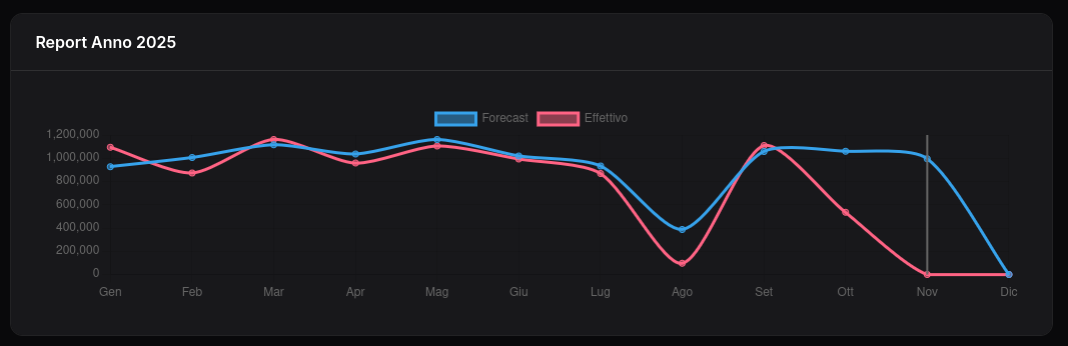
\includegraphics[width=\textwidth]{img/previsione_2025.png}
    \caption{Andamento storico vs previsioni annuali (screenshot della dashboard)}
    \label{fig:forecast-annual}
\end{figure}
\begin{figure}[H]
    \centering
    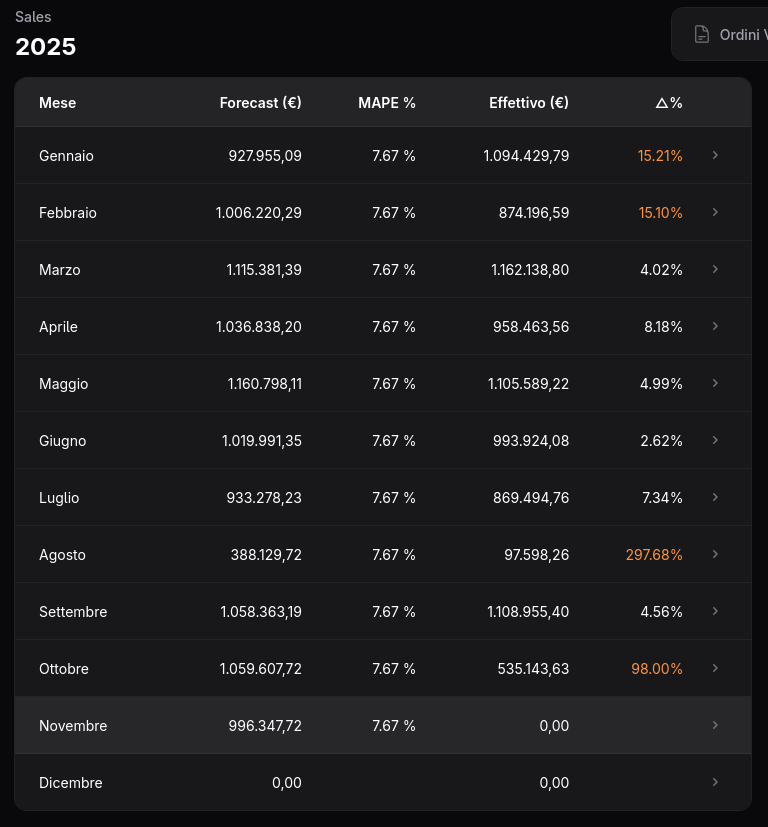
\includegraphics[width=0.9\textwidth]{img/tabella_previsione_2025.png}
    \caption{Tabella di dettaglio delle previsioni annuali}
    \label{fig:forecast-annual-table}
\end{figure}

\subsection{Feature più influenti}
L’analisi SHAP mette in evidenza le variabili che guidano maggiormente le previsioni. Nel grafico, ogni punto rappresenta un campione: i colori indicano il valore della feature (rosso = valore alto, blu = valore basso), mentre la posizione sull’asse orizzontale misura il contributo SHAP (a destra aumenta la previsione, a sinistra la riduce). La densità dei punti lungo l’asse mostra la distribuzione degli impatti.
Alcune delle feature più influenti sono:
\begin{itemize}
    \item \texttt{quantity\_roll\_med6}: media mobile a 6 periodi sulle quantità vendute; valori alti spostano nettamente a destra, segno che volumi recenti elevati trainano la domanda attesa.
    \item \texttt{article\_avg\_monthly\_sale}: media mensile storica per articolo; contribuisce positivamente quando sopra la media, stabilizzando le previsioni su trend consolidati.
    \item \texttt{sales\_history\_ratio}: rapporto tra vendite recenti e storiche; valori alti indicano accelerazione e portano contributi positivi, mentre valori bassi riducono la stima.
    \item \texttt{summer\_shutdown}: flag di chiusura estiva (es. agosto); i punti rossi a sinistra mostrano che quando la chiusura è attiva la previsione cala, come atteso per lo stop produttivo.
\end{itemize}
\begin{figure}[H]
    \centering
    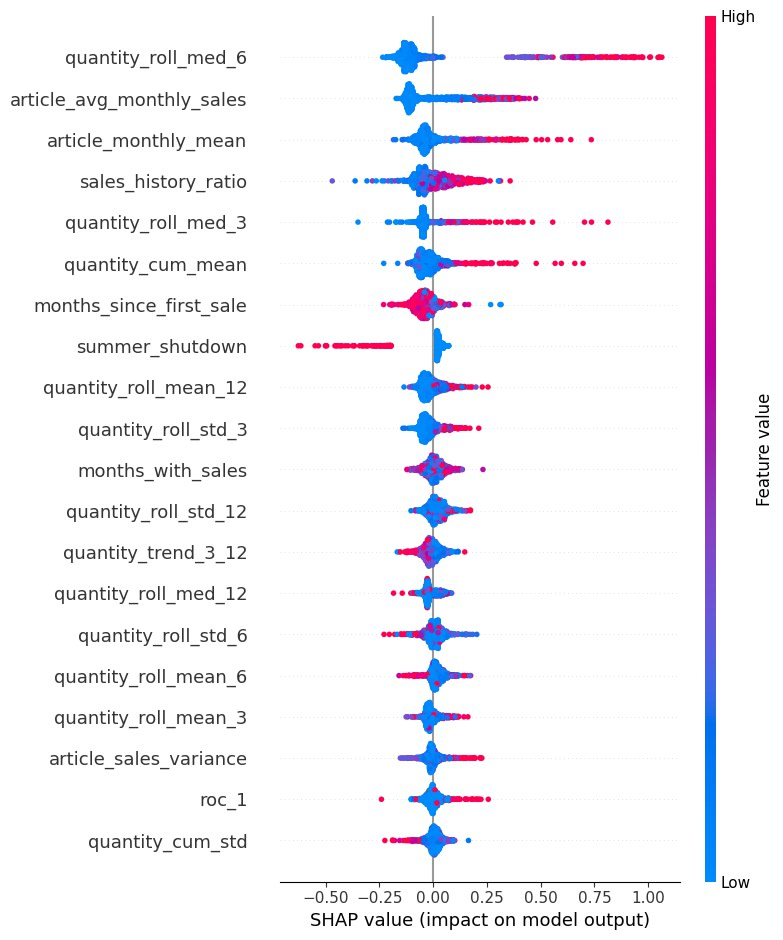
\includegraphics[width=0.95\textwidth]{img/shap_valori.png}
    \caption{Feature più influenti secondo SHAP (valori e segno del contributo)}
    \label{fig:feature-importance}
\end{figure}
\subsection{Miglioramenti futuri}
Nonostante i risultati positivi, ci sono margini di miglioramento per affrontare alcune criticità emerse:
\begin{itemize}
    \item \textbf{Previsioni per singoli articoli}: per quanto l'andamento generale sia buono, le previsioni a livello di singolo articolo mostrano scostamenti più marcati suprattutto per articoli con bassa storicità o stagionalità irregolare. Si prevede di integrare modelli specifici per cluster di articoli simili.
    \item \textbf{Automazione scelta iperparametri}: attualmente l'ottimizzazione degli iperparametri del modello XGBoost è manuale e richiede tempo. L'implementazione di tecniche di AutoML potrebbe velocizzare questo processo e migliorare le performance.
    \item \textbf{Automazione scelta feature}: l'attuale selezione delle feature si basa su analisi statistiche preliminari. L'adozione di metodi automatici di feature selection potrebbe identificare variabili più rilevanti e ridurre il rumore nei dati.
\end{itemize}

\section{Valutazione personale}
Durante lo stage ho avuto l'opportunità di applicare e approfondire diverse competenze tecniche acquisite durante il percorso universitario, in particolare nell'ambito del machine learning, della gestione di progetti software e dell'implementazione di pratiche DevOps come il testing automatizzato e la continuous integration. Ho imparato a lavorare in un contesto professionale, collaborando con un team eterogeneo e affrontando sfide reali legate alla gestione dei dati e alla scalabilità delle soluzioni. 
Questo stage ha rappresentato un'importante esperienza di crescita personale e professionale, che mi ha permesso di consolidare le mie conoscenze e di acquisire nuove competenze utili per il mio futuro lavorativo.

Per quanto riguarda il progetto sviluppato, ritengo che abbia raggiunto gli obiettivi prefissati, fornendo una soluzione efficace per la previsione della domanda e contribuendo al miglioramento dei processi decisionali dell'azienda.
Sono consapevole che ci sono ancora margini di miglioramento e che il progetto potrà evolversi ulteriormente in futuro, ma sono soddisfatto del lavoro svolto e dei risultati ottenuti fino ad ora.

\newpage
